%=============================================================================%
% Author: 	John Joseph Valletta
% Date: 	11/04/2019
% Title: 	Fews slides on practical issues/tips
%=============================================================================%

% Preamble
 \documentclass[pdf]{beamer}
\usepackage[export]{adjustbox}
\usepackage{framed}
\usepackage{color}
\definecolor{dkgreen}{rgb}{0,0.6,0}
\definecolor{gray}{rgb}{0.5,0.5,0.5}
\definecolor{mauve}{rgb}{0.58,0,0.82}
\definecolor{deepblue}{rgb}{0,0,0.5}
\definecolor{deepred}{rgb}{0.6,0,0}
\definecolor{deepgreen}{rgb}{0,0.5,0}
\definecolor{lightgray}{rgb}{0.92,0.92,0.92}
\definecolor{myblue}{rgb}{0.12, 0.47, 0.71} 
\definecolor{tealblue}{rgb}{0, 0.5, 0.5}
\usepackage{listings} % to insert code
\usepackage{textpos} % textblock
\usepackage{verbatim}
\usepackage{hyperref}
\hypersetup{colorlinks=true, urlcolor=blue, linkcolor=black} 

% Presentation configuration
\mode<presentation>{\usetheme{Madrid}}
\usecolortheme[named=myblue]{structure}
\useinnertheme{circles} % circles, rectanges, rounded, inmargin
\usefonttheme[onlymath]{serif} % makes math fonts like the usual LaTeX ones
\setbeamercovered{transparent=4} % transparent
\setbeamertemplate{caption}{\raggedright\insertcaption\par} % Remove the word "Figure" from caption %\setbeamertemplate{caption}[default]
\setbeamertemplate{navigation symbols}{} % don't put navigation tools at the bottom (alternatively \beamertemplatenavigationsymbolsempty)
\graphicspath{ {./img/} }

% Titlepage
\title[Practical issues and tips]{Practical issues and tips}
\subtitle{(avoid machine learning going mad)}
\author{John Joseph Valletta}
\date[April 2019]{April 2019}
\institute[]{University of Exeter, Penryn Campus, UK}
\titlegraphic{
\hfill

\includegraphics[width=\textwidth, keepaspectratio]{logo.jpg}}

%=============================================================================%
%=============================================================================%
% Start of Document
%=============================================================================%
%=============================================================================%
\begin{document}

%=============================================================================%
%=============================================================================%
\begin{frame}
\titlepage
\end{frame}

%=============================================================================%
%=============================================================================%
\begin{frame}{Overview}
\begin{itemize}\addtolength{\itemsep}{1.5\baselineskip}
	\item Feature selection
	\item The wrong way to do cross-validation
	\item Imbalanced data
	\item Machine learning gone mad
	\item Practical tips in machine learning
\end{itemize}
\end{frame}

%=============================================================================%
%=============================================================================%
\begin{frame}{Feature selection}
Often one wants to determine \textbf{which} features are best at predicting the 
outcome. There are three main types of feature selection methods:
\vfill
\begin{enumerate}\addtolength{\itemsep}{1.5\baselineskip}
	\item<2-> \textbf{Filter}: Use univariate measures (e.g correlation) to assess the feature's relevance
	\item<3-> \textbf{Wrapper}: Employ a greedy strategy to search for the best subset of features (e.g. stepwise selection)
	\item<4-> \textbf{Embedded}: Feature selection is an implicit aspect of the learning alogrithm (e.g. LASSO)
\end{enumerate} 
\end{frame}

%=============================================================================%
%=============================================================================%
\begin{frame}{The wrong way to do cross-validation}

\begin{columns}

\begin{column}{0.4\textwidth}
	\begin{center}
   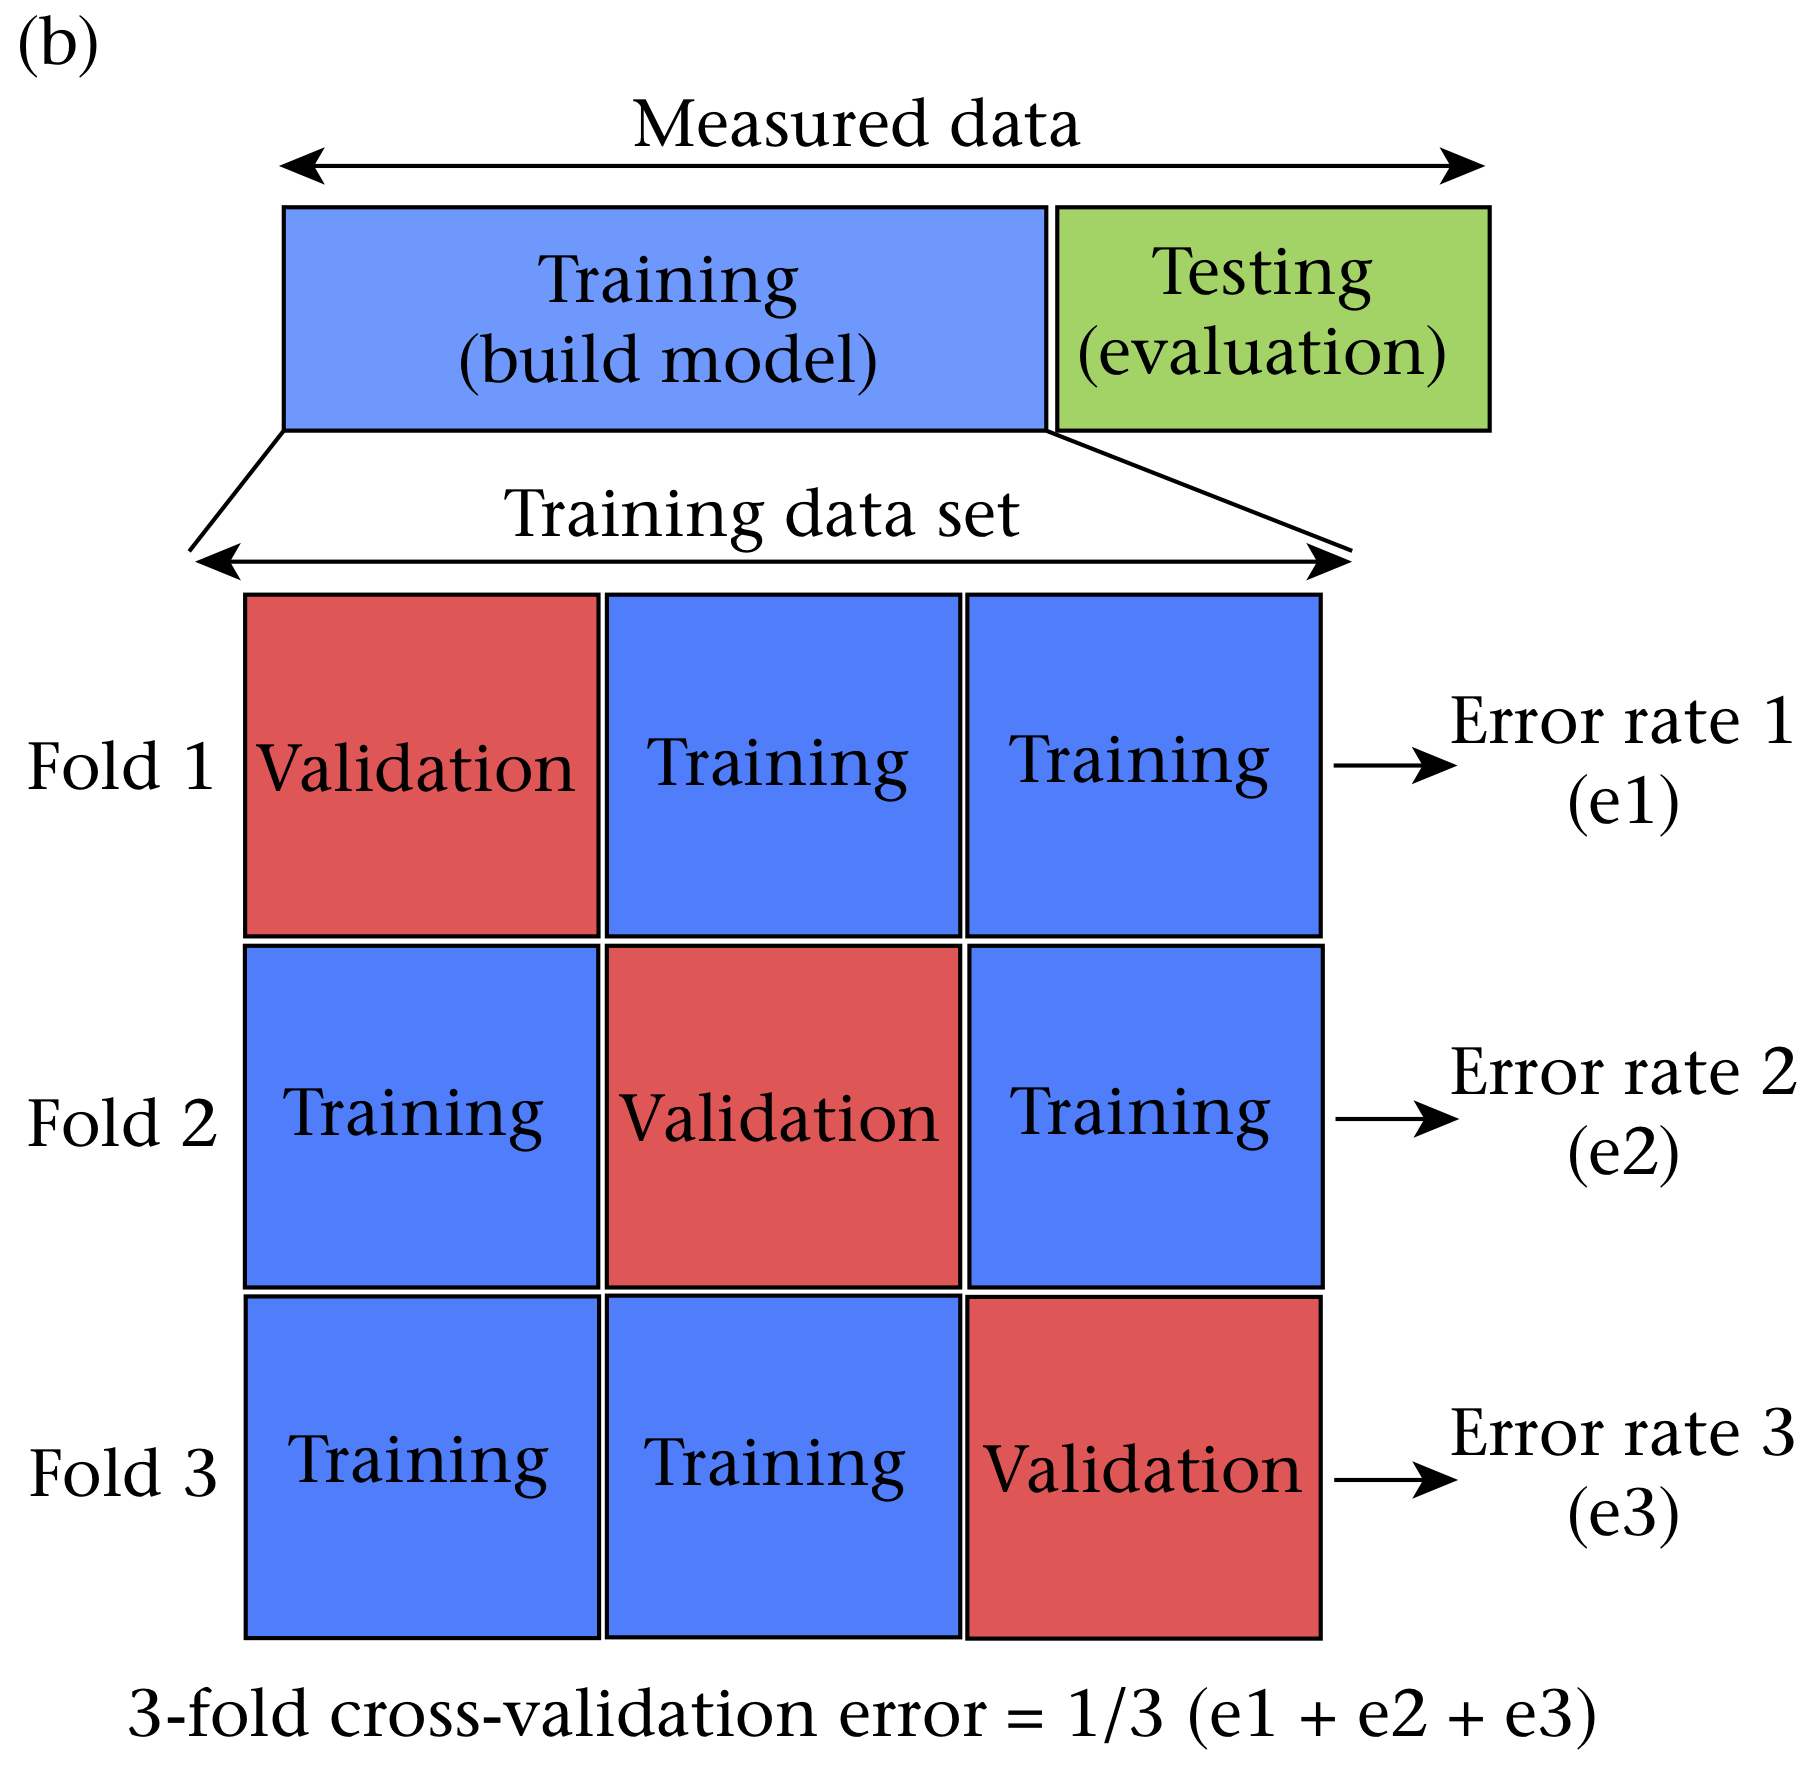
\includegraphics[width=.9\textwidth]{crossvalidation.png}
   \end{center}
\end{column}

\begin{column}{0.6\textwidth}
	\begin{enumerate}\addtolength{\itemsep}{1\baselineskip}
		\item Filter out features by their univariate association with the outcome using all of the training data
		\item Use the selected features to build a predictive model
		\item Employ $k$-fold cross-validation to tune the hyperparameters and estimate predictive performance
	\end{enumerate}
\end{column}

\end{columns}
\vfill
{\tiny See Section 7.10.2 of ``The Elements of Statistical Learning" by T. Hastie, R. Tibshirani and J. Friedman}
\end{frame}

%=============================================================================%
%=============================================================================%
\begin{frame}{The right way to do cross-validation}

\begin{columns}

\begin{column}{0.4\textwidth}
	\begin{center}
   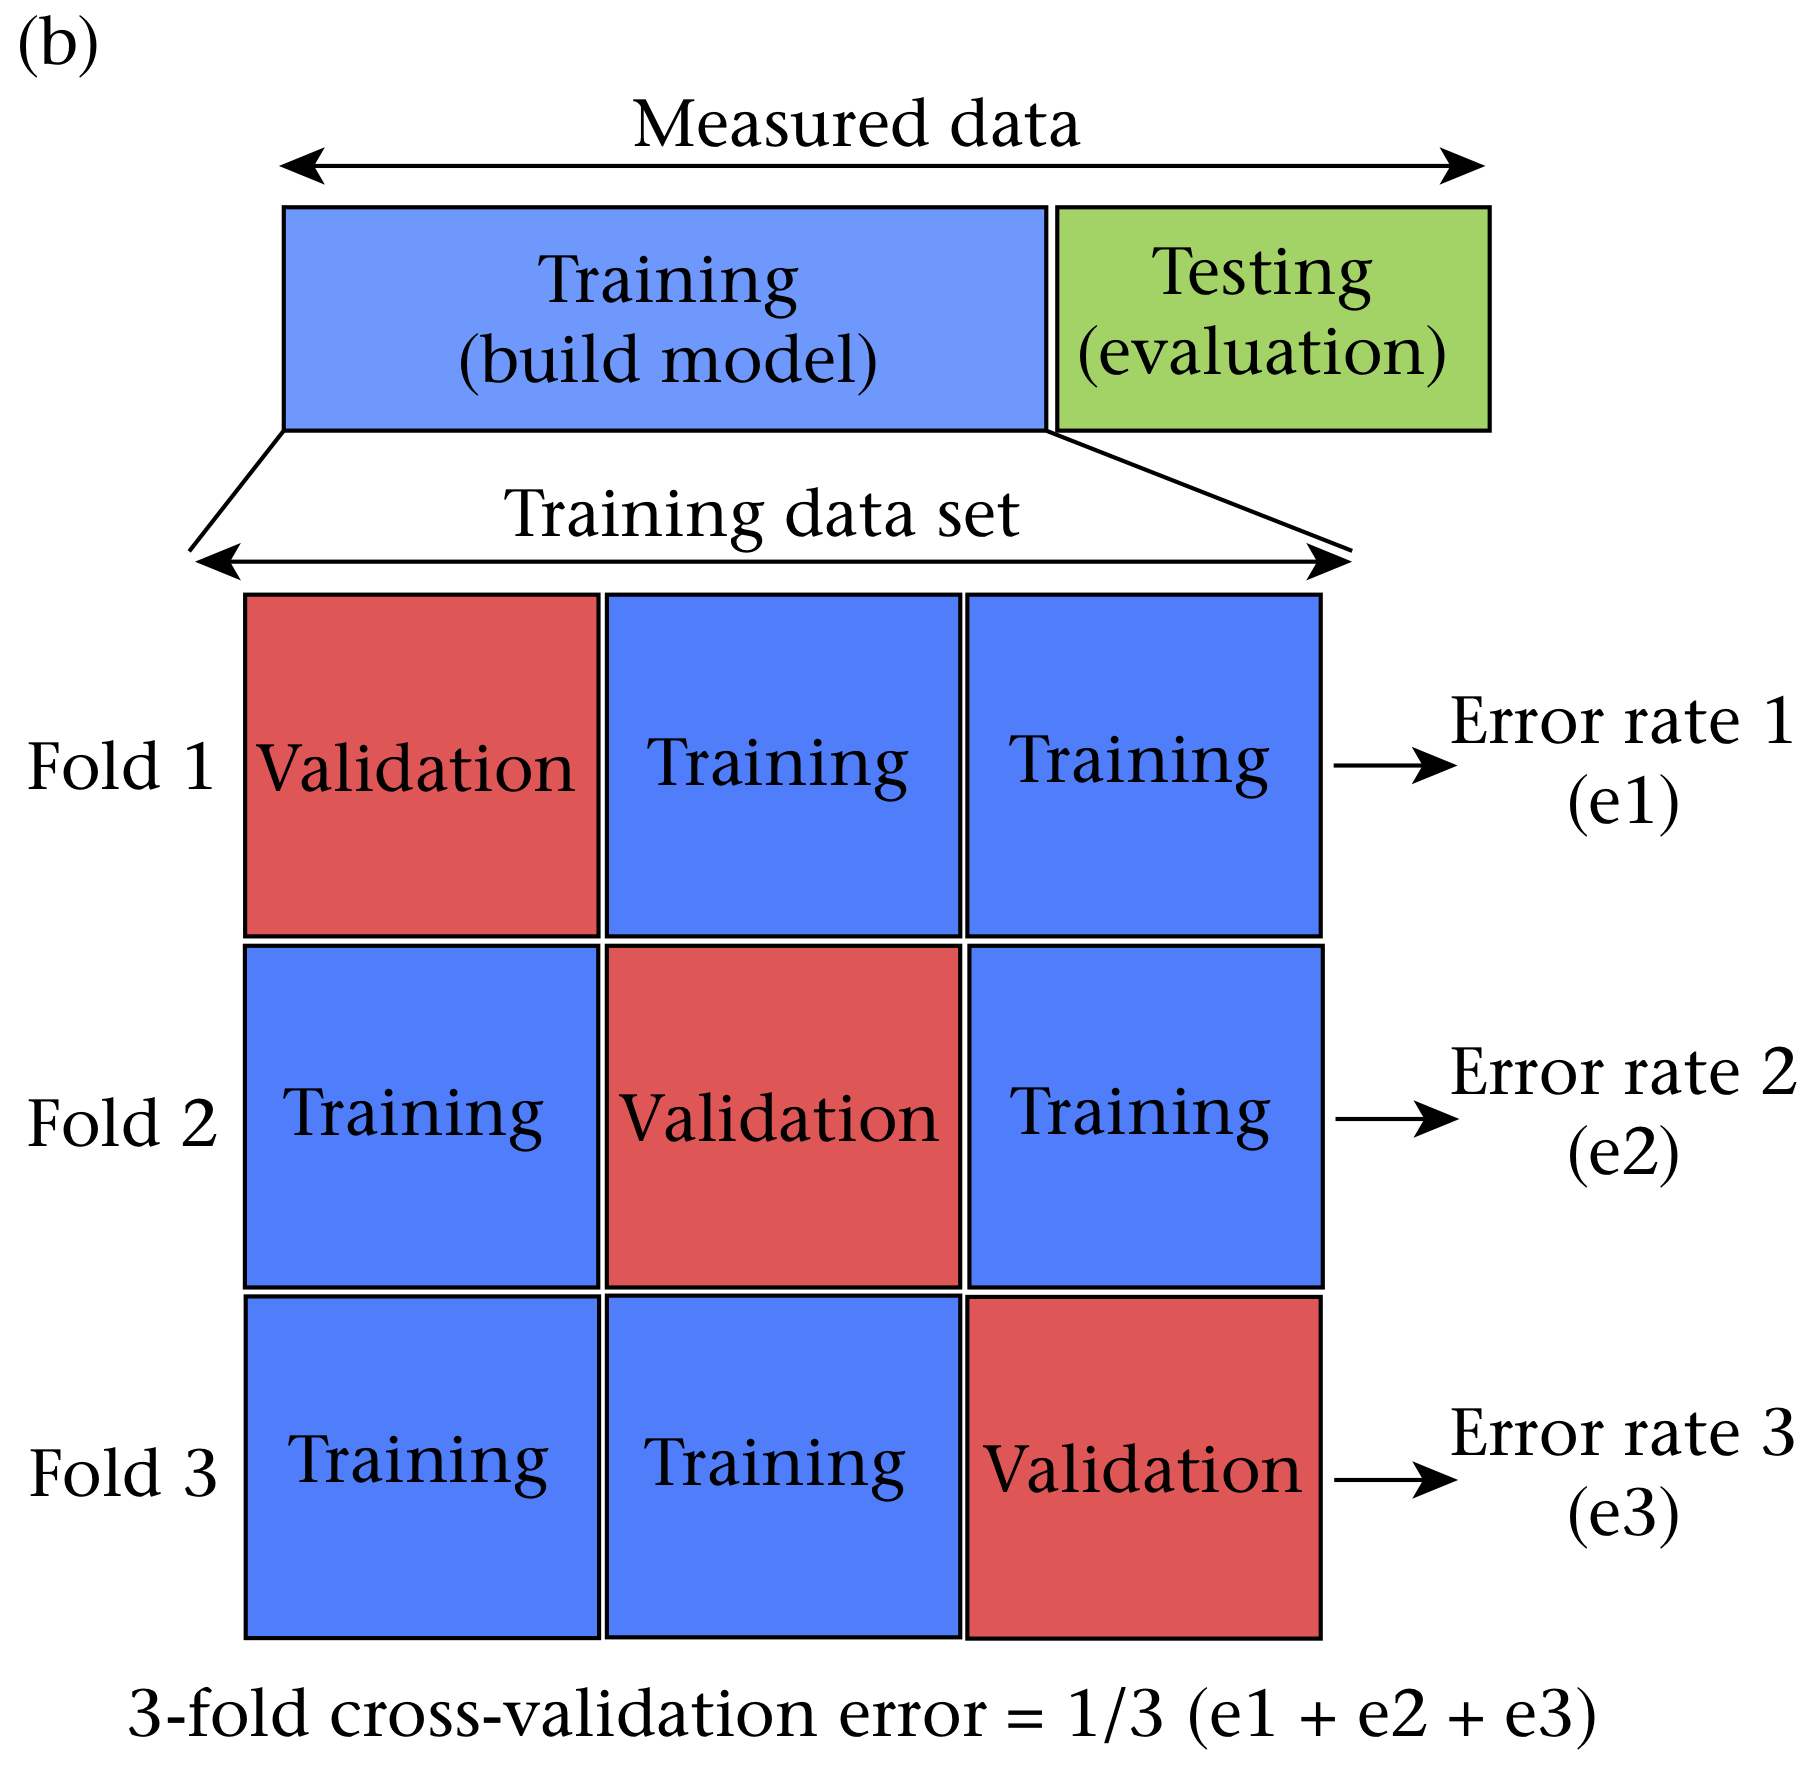
\includegraphics[width=.9\textwidth]{crossvalidation.png}
   \end{center}
\end{column}

\begin{column}{0.6\textwidth}
	\begin{enumerate}\addtolength{\itemsep}{1\baselineskip}
		\item Filter out features by their univariate association with the outcome using all of the training data, \textbf{except} those in fold $k$
		\item Use the selected features to build a predictive model using all of the training data \textbf{except} those in fold $k$ 
		\item Use the model to predict the outcome for fold $k$ to estimate the predictive accuracy
	\end{enumerate}
\end{column}

\end{columns}
\vfill
{\tiny See Section 7.10.2 of ``The Elements of Statistical Learning" by T. Hastie, R. Tibshirani and J. Friedman}
\end{frame}

%=============================================================================%
%=============================================================================%
\begin{frame}{Imbalanced data}
\begin{itemize}\addtolength{\itemsep}{3\baselineskip}
	\item<1-> \textbf{Imbalanced data} arises in applications where one class dominates over the other. For example:
	\begin{itemize}\addtolength{\itemsep}{.8\baselineskip}
		\item Easier to collect ``healthy'' samples than rare disease ones
		\item Legitimate transactions far outweight the fraudelent ones
	\end{itemize}
	\item <2-> \textbf{Balancing} the class distribution through \textbf{resampling} is one of the most popular solutions:
	\begin{itemize}\addtolength{\itemsep}{.8\baselineskip}
		\item<3-> \textbf{Undersampling}: Put to one side observations from the \textit{majority} class
		\item<4-> \textbf{Oversampling}: Replicate observations from the \textit{minority} class 
	\end{itemize}
\end{itemize}
\end{frame}

%=============================================================================%
%=============================================================================%
\begin{frame}{Machine learning gone mad - The US tank experiment}
\begin{itemize}\addtolength{\itemsep}{0.5\baselineskip}
	\item<1-> 1980s: Pentagon got excited about artificial neural networks
	\item<2-> Wanted a classifier to detect whether a tank is hiding behind trees
	\item<3-> Collected photos of trees with/without tanks hiding in them
	\item<4-> Trained neural network performed \textit{excellently} on the testing dataset\\
	\textbf{Champagne to all the scientists!}
\end{itemize}
\begin{center}
		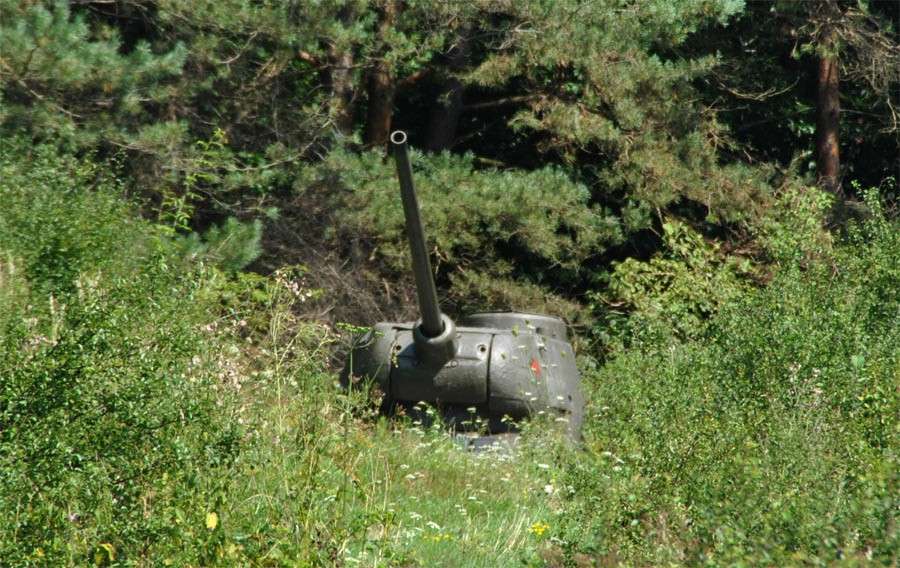
\includegraphics[width=0.45\textwidth]{tank.jpg}
\end{center}
\end{frame}

%=============================================================================%
%=============================================================================%
\begin{frame}{Machine learning gone mad - The US tank experiment}
\begin{itemize}\addtolength{\itemsep}{0.5\baselineskip}
	\item<1-> Another set of tank/no tank photos was commissioned
	\item<2-> The classifier was now useless and no better than randomly guessing
	\item<3-> Someone noted that all previous photos were taken on:
	\begin{description}
		\item[no tank:] \textbf{sunny blue} skies day
		\item[tank:] \textbf{cloudy grey} skies day
	\end{description}
	\item<4-> Neural network had learnt whether it was a sunny or cloudy day\\
	\textbf{God bless the United States of America!}
\end{itemize}	
\begin{center}
		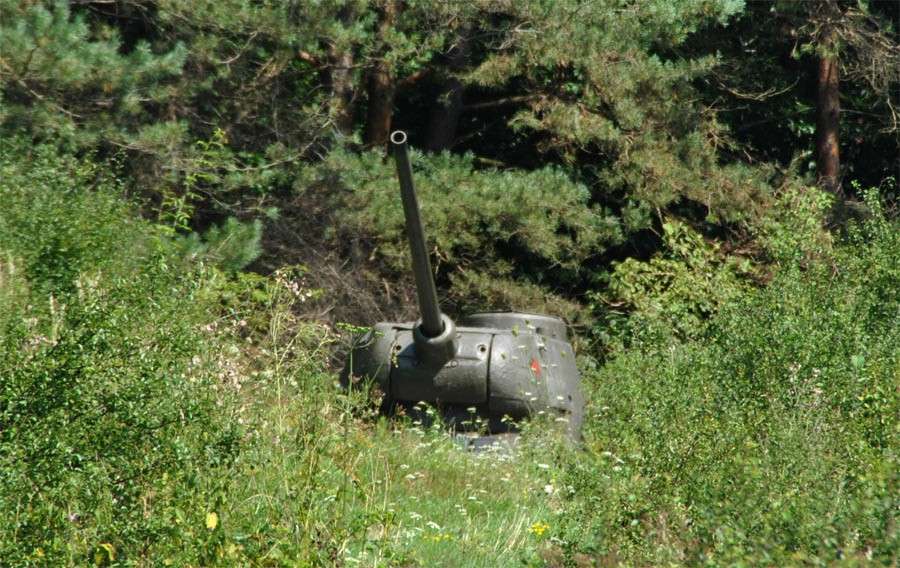
\includegraphics[width=0.45\textwidth]{tank.jpg}
\end{center}
\end{frame}	

%=============================================================================%
%=============================================================================%
\begin{frame}{Machine learning gone mad - Google flu trends}
\begin{itemize}\addtolength{\itemsep}{1\baselineskip}
	\item<1-> 2008: Google decided to showcase the power of big data 
	\item<2-> Built a predictive model to estimate influenza activity	
	\item<3-> Training data were queries containing terms such as cough and fever
	\item<4-> Used IP address to break data by states
	\item<5-> Outcome (label) was influenza-like illness (ILI) physician visits collected by the CDC 
	(Centers for Disease Control and Prevention)
	\item<6-> Model was successful, it predicted a spike in the mid-Atlantic region of the US two weeks prior to the CDC\\
	\textbf{Google is great!}
\end{itemize}
\end{frame}

%=============================================================================%
%=============================================================================%
\begin{frame}{Machine learning gone mad - Google flu trends}
\begin{center}
		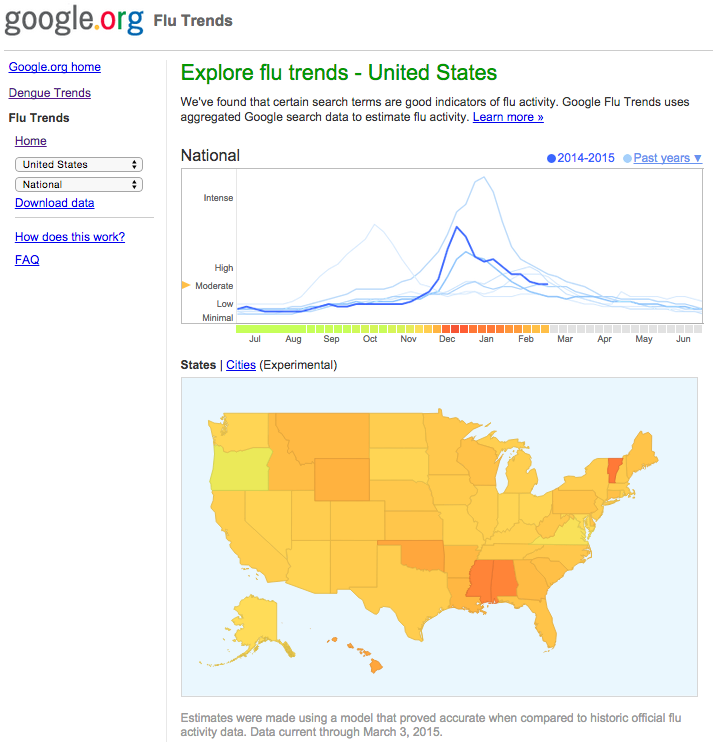
\includegraphics[width=0.6\textwidth]{googleFluTrend1.png}
\end{center}
\end{frame}

%=============================================================================%
%=============================================================================%
\begin{frame}{Machine learning gone mad - Google flu trends}
\begin{center}
		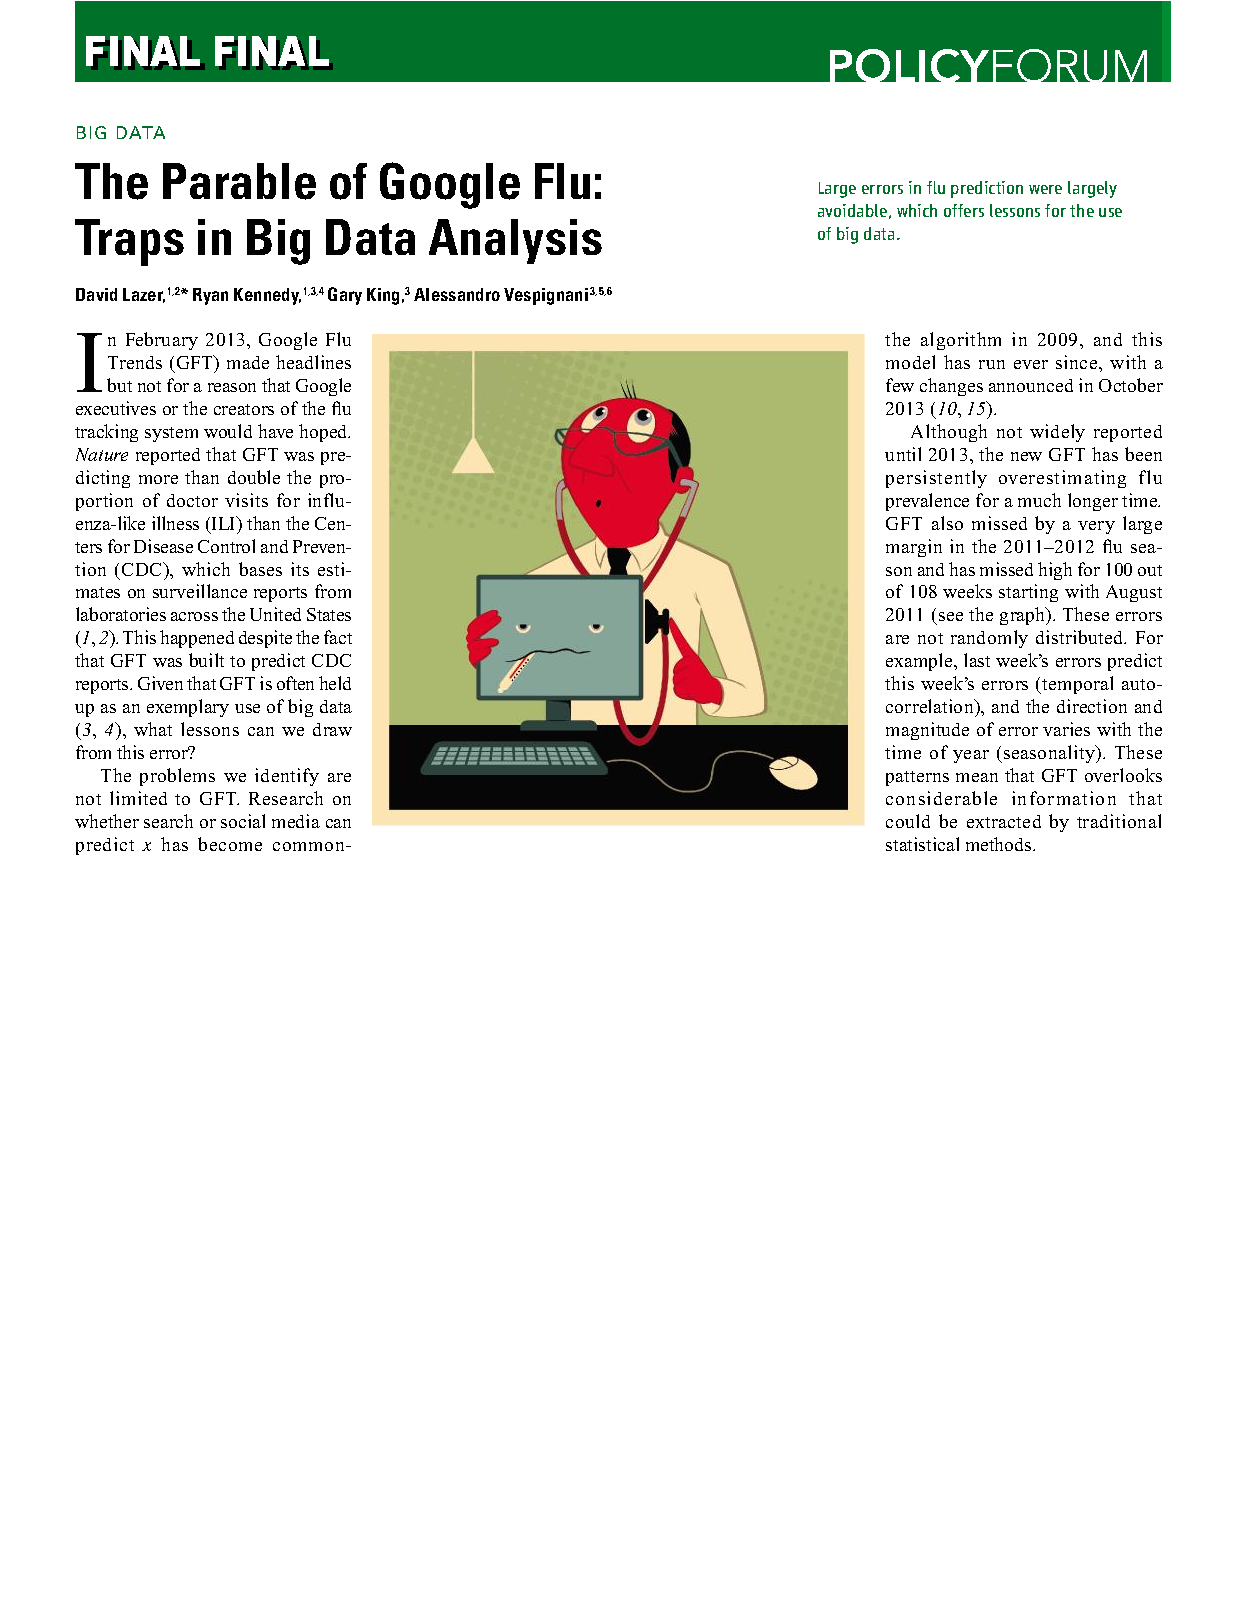
\includegraphics[width=0.8\textwidth]{googleFluTrend2.pdf}
\end{center}
\end{frame}

%=============================================================================%
%=============================================================================%
\begin{frame}{Machine learning gone mad - Google flu trends}
\begin{center}
		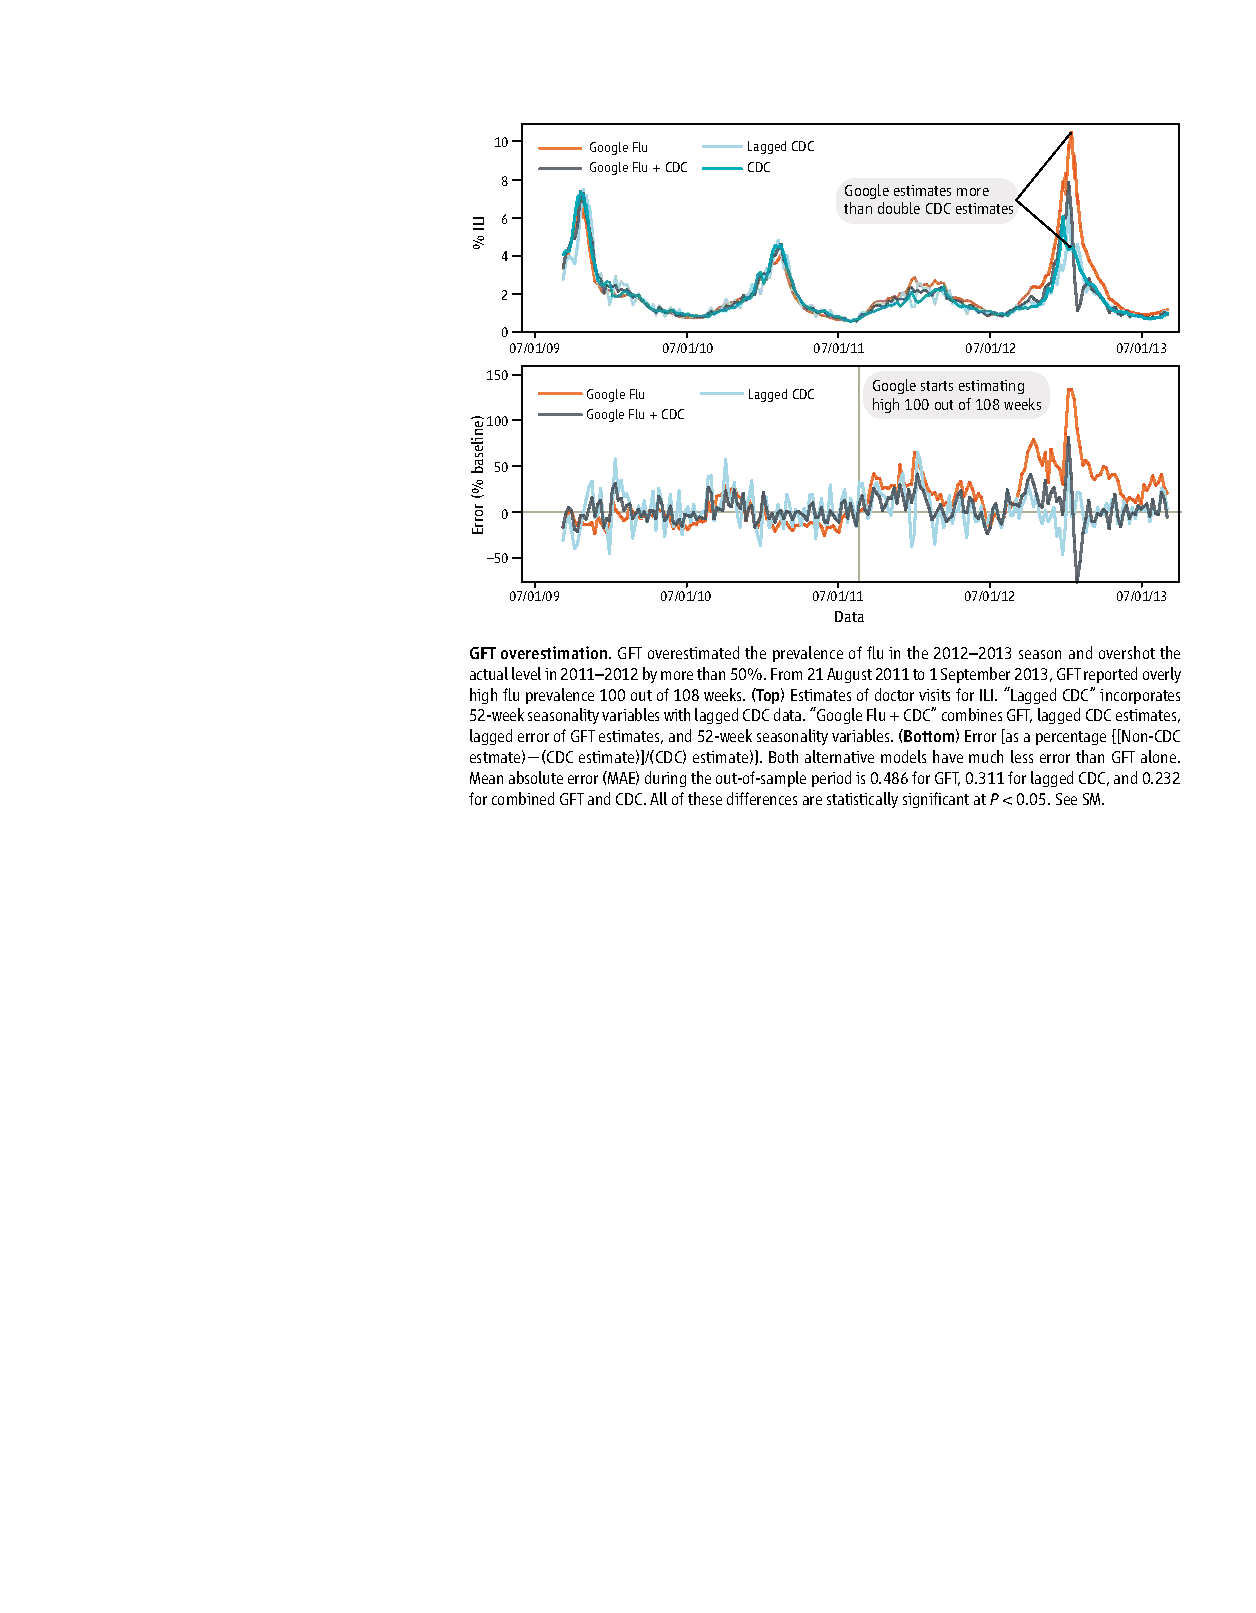
\includegraphics[width=0.65\textwidth]{googleFluTrend3.pdf}
\end{center}
\end{frame}

%=============================================================================%
%=============================================================================%
\begin{frame}{Google flu trends, so what went wrong?}
\begin{itemize}\addtolength{\itemsep}{.75\baselineskip}
	\item<1-> Google had to mine 50 million search terms that best correlated with 1,152 ``true'' data points 
	collected by CDC (Centers for Disease Control and Prevention). They retained 45 queries 
	\item<2-> Winter is coming: Correlation is not causation
	\item<3-> Are these correlates stable and comparable over time?
	\item<4-> Google's search algorithm changes very frequently. Autosuggest feature might have implicitly 
	caused more people to search flu-related terms 
	\item<5-> Is it time to recalibrate the model and/or hybridise both data sources?
	\item<6-> In 2014, Google retrained and updated the model significantly, but cancelled the project in 2015
\end{itemize}
\end{frame}

%=============================================================================%
%=============================================================================%
\begin{frame}{Laws of data analysis}
\begin{enumerate}\addtolength{\itemsep}{1.5\baselineskip}
	\item<2-> Shite in, shite out\\
			\textit{Anonymous}
	\item<3-> If you torture the data long enough it will confess to anything\\
			\textit{Ronald Coase} (1910 - 2013)
	\item<4-> A sufficiently elaborate analysis process can always lend an air of legitimacy\\ 
			\textit{Chris Laws, ex-McLaren boss} 
\end{enumerate}
\end{frame}

%=============================================================================%
%=============================================================================%
\begin{frame}{A few important tips}
\begin{itemize}\addtolength{\itemsep}{0.5\baselineskip}
	\item<2-> \textbf{Data exploration} is key to understanding the data's structure. Use 
	dimensionality reduction techniques to visualise high-dimensional data 
	\item<3-> Features with \textbf{little variability} can be safely ignored
	\item<4-> \textbf{Impute}/ignore missing data (are they missing completely at random?)
	\item<5-> \textbf{Standardise}/\textbf{normalise} features with widely varying ranges
	\item<6-> \textbf{Features} extracted from the data need to be directly relevant to the question
	you're asking
	\item<7-> Use \textbf{expert application knowledge} where possible over automatic feature extraction 
	\item<8-> \textbf{Do not} trust predictions for inputs outside the training dataset range 
	(i.e avoid extrapolation)
\end{itemize}
\end{frame}

%=============================================================================%
%=============================================================================%
\begin{frame}{Practical advice}
\begin{itemize}
	\item Your fitted predictive model has poor accuracy on the testing data\\What should you do next?
\end{itemize}
\vfill
\begin{columns}
\begin{column}{0.45\textwidth}
	\visible<2->{
	Recall the bias-variance tradeoff:
	\begin{center}
			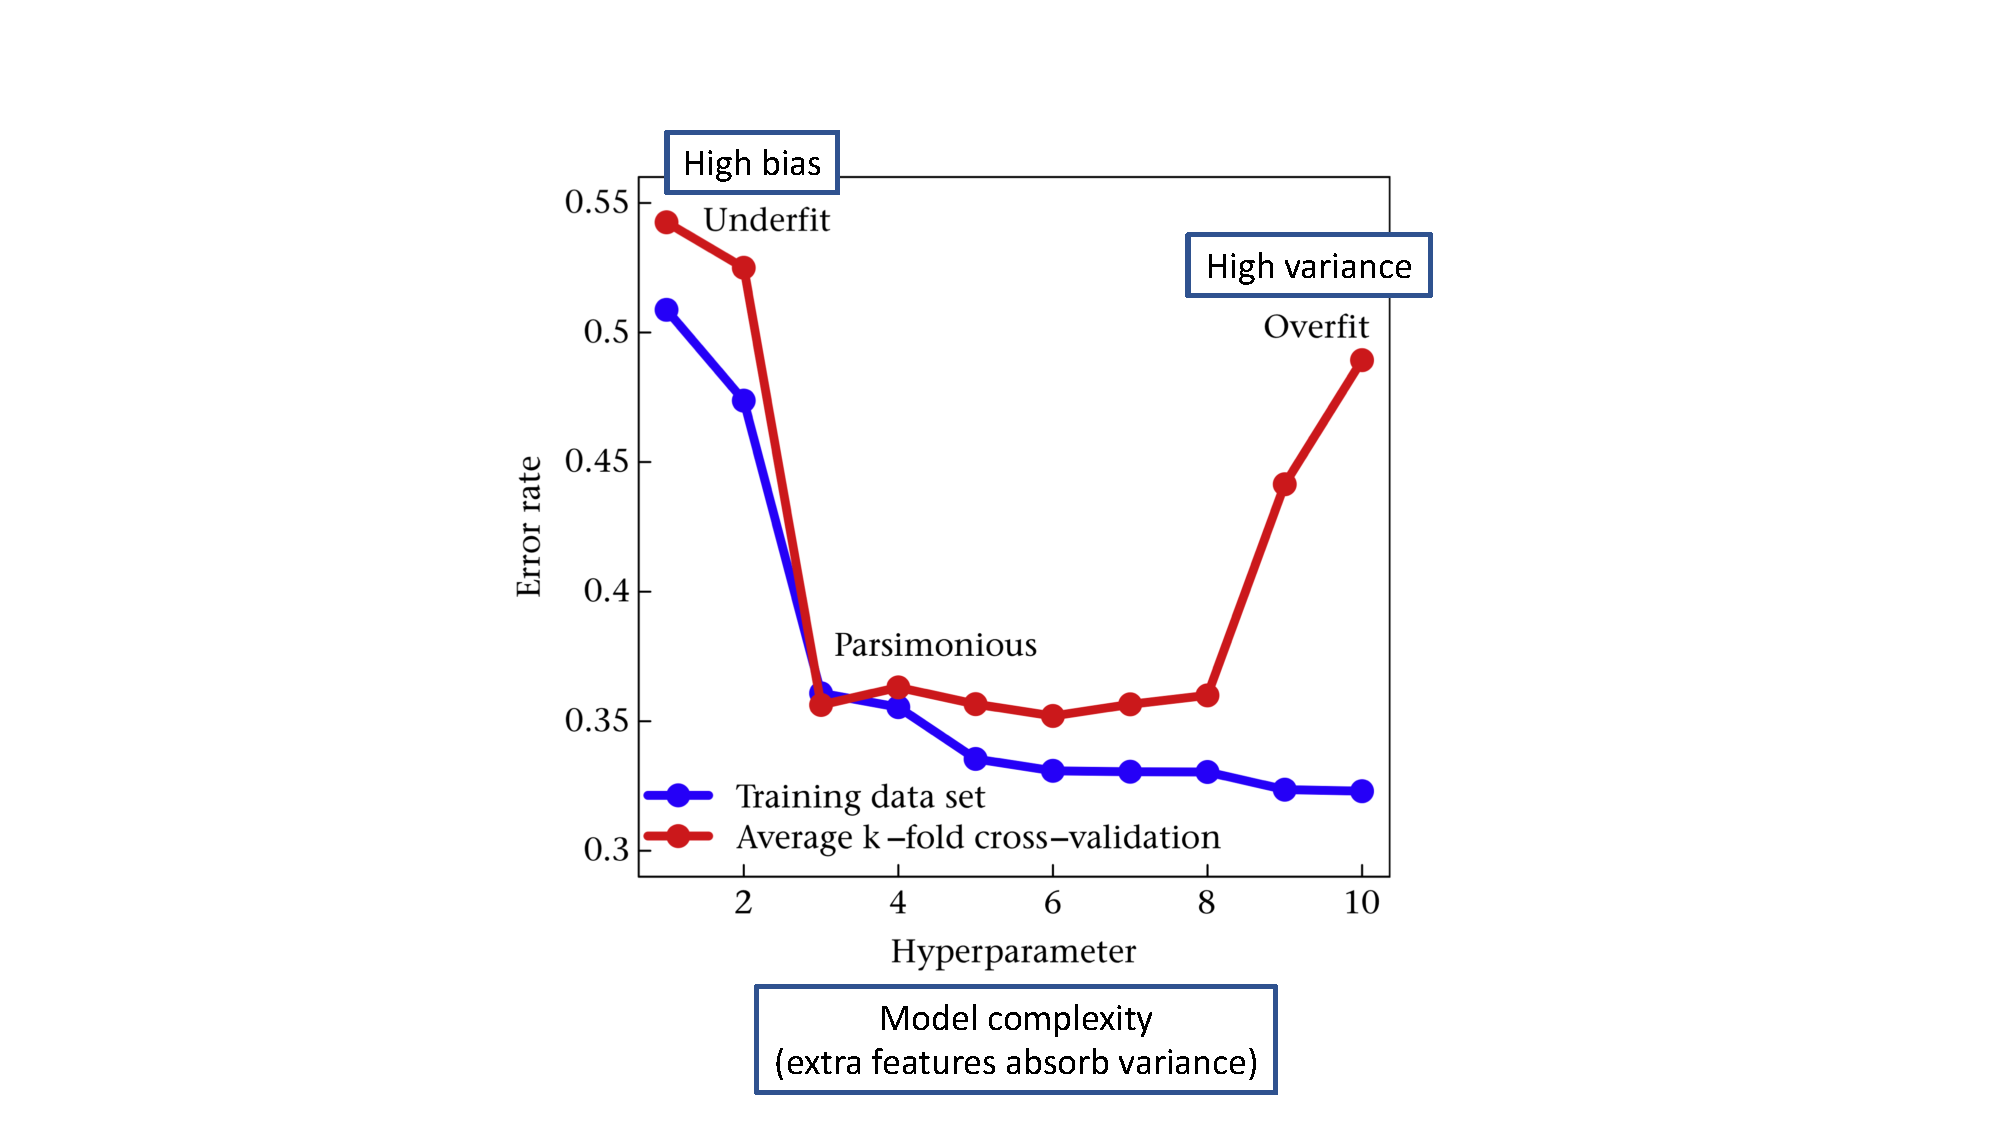
\includegraphics[width=.9\textwidth]{biasvariance.pdf}
	\end{center}}
\end{column}
\begin{column}{0.55\textwidth}
	\begin{enumerate}\addtolength{\itemsep}{1\baselineskip}
		\item<3-> \textbf{High bias/underfit}\\ Training \textit{and} validation errors are large
		\item<4-> \textbf{High variance/overfit}\\ Validation error $\gg$ Training error
	\end{enumerate}
\end{column}

\end{columns}

\end{frame}

%=============================================================================%
%=============================================================================%
\begin{frame}{Learning curves}
\begin{itemize}\addtolength{\itemsep}{0.5\baselineskip}
	\item \textbf{Learning curves} are useful diagnostic plots for learning algorithms
	\item It's a plot of model performance/error rate vs experience/sample size
\end{itemize} 
\vfill
\begin{center}
		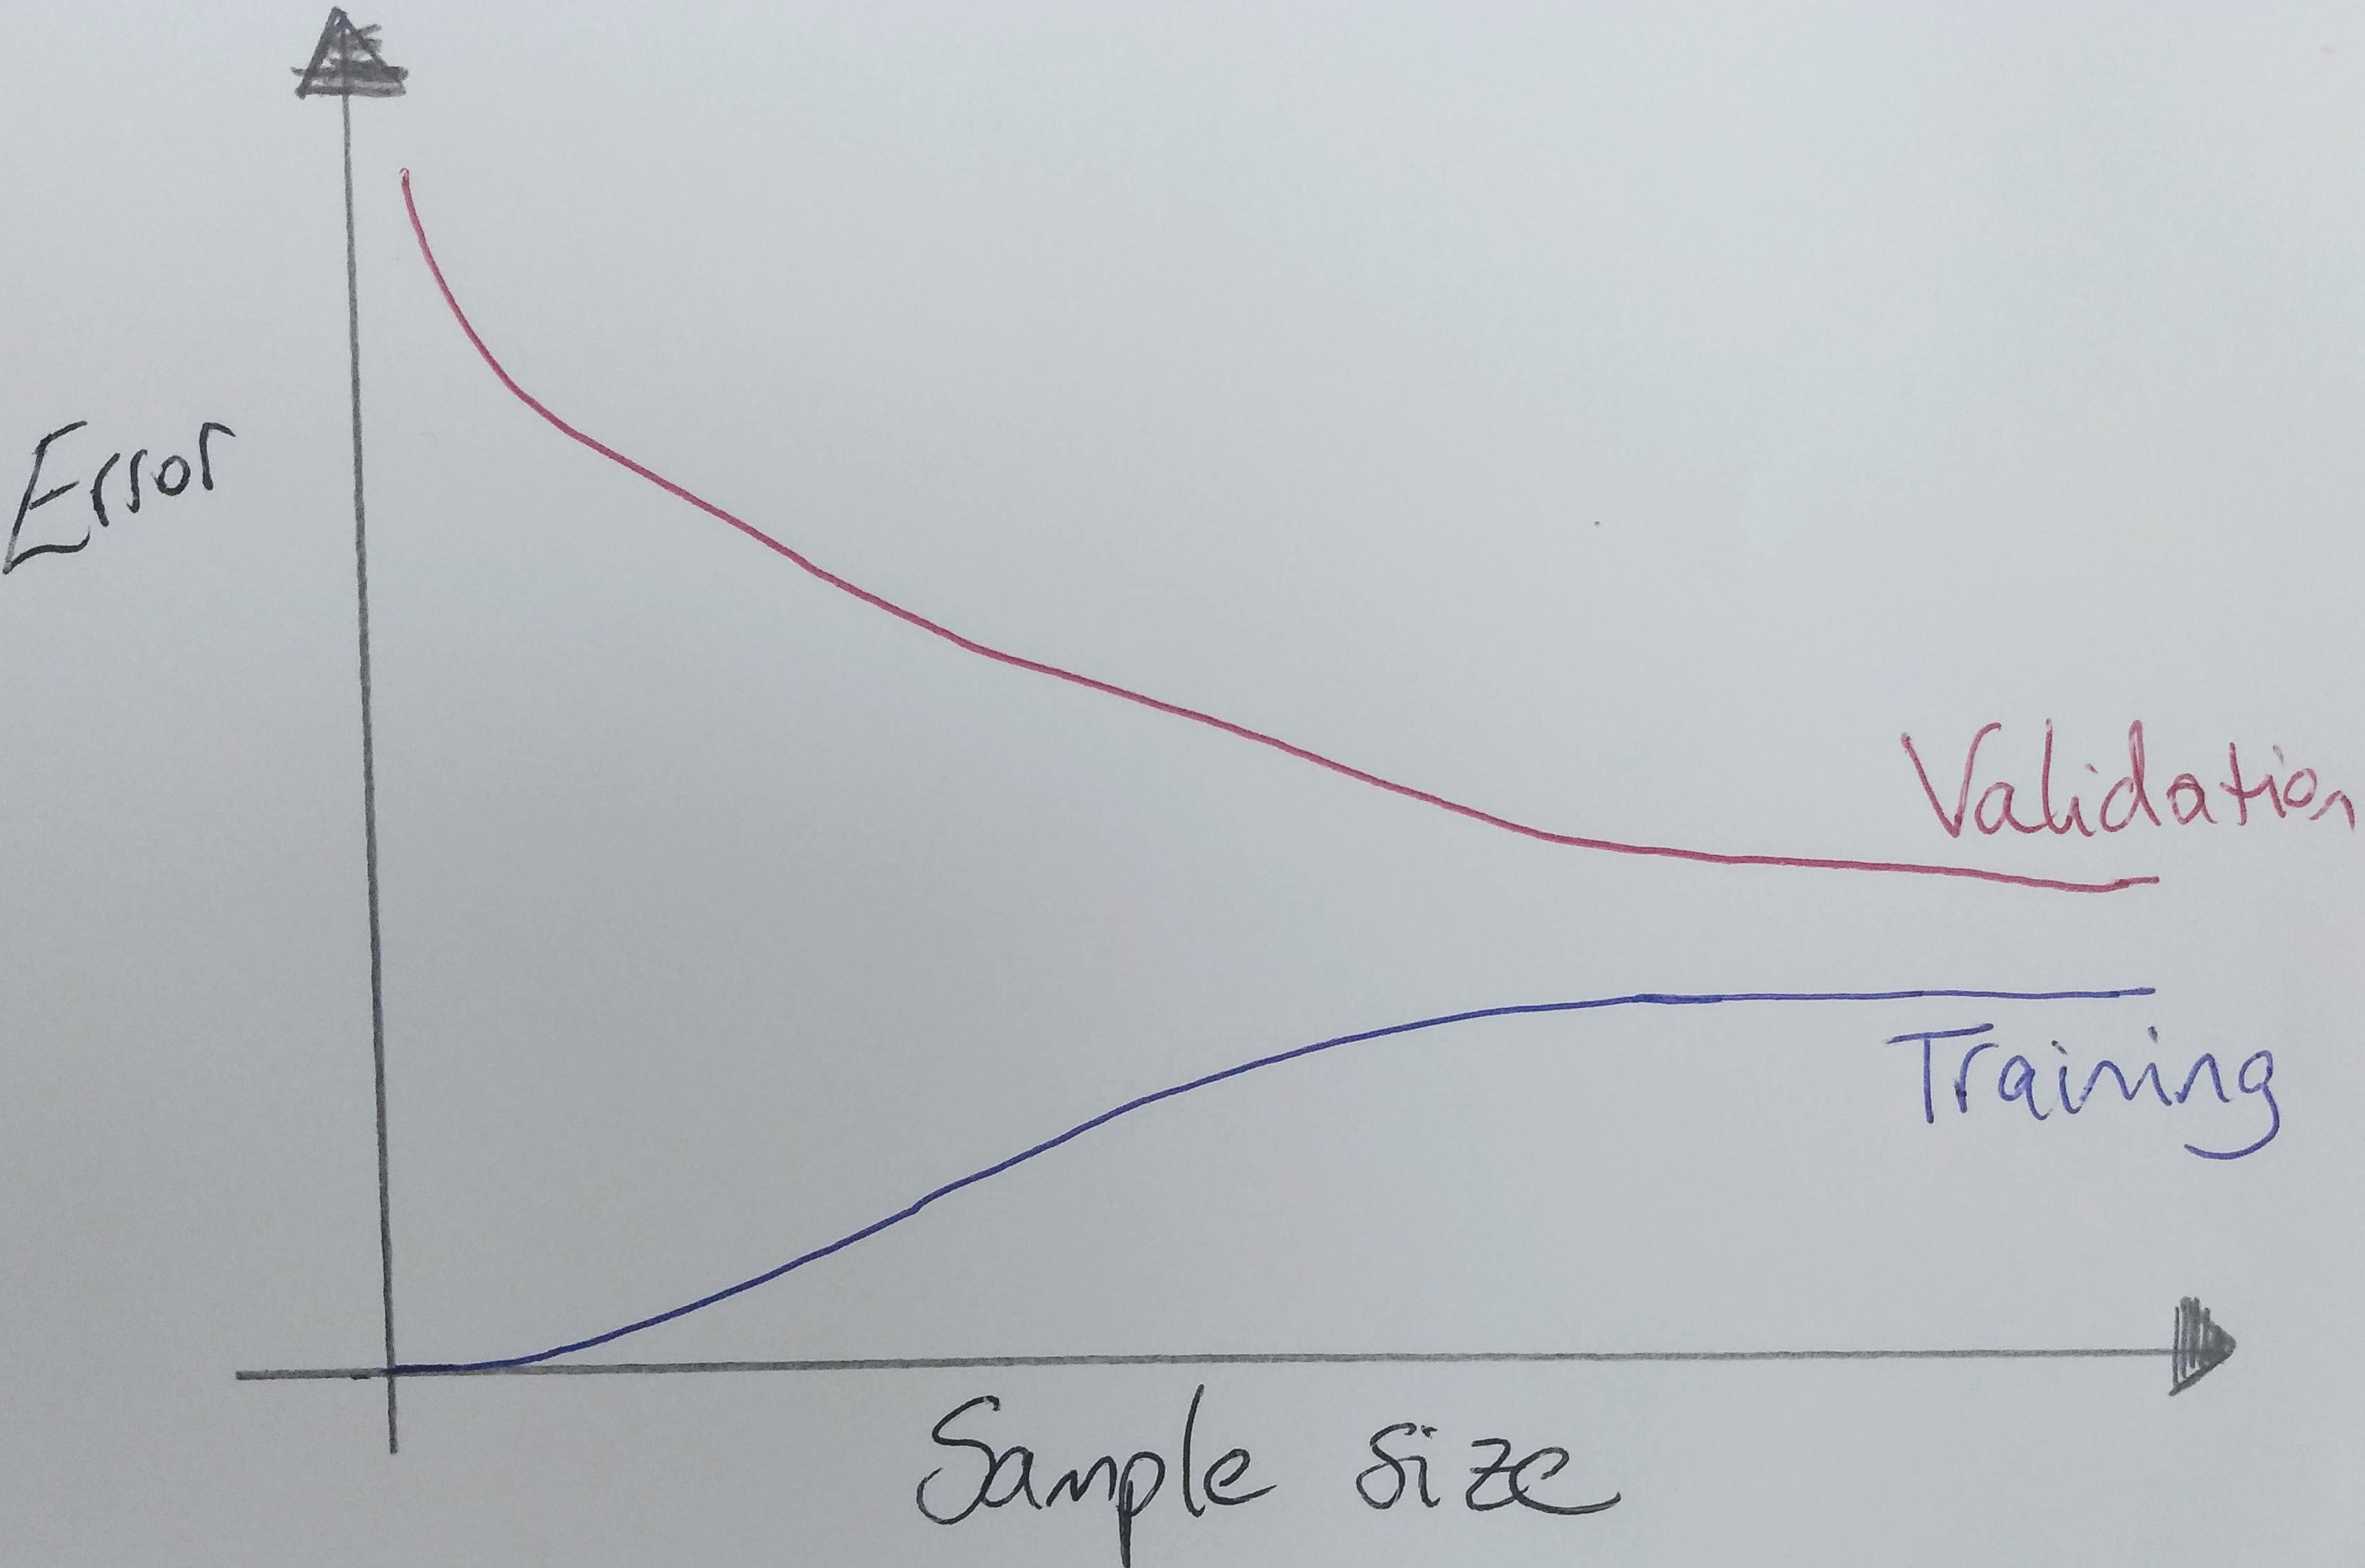
\includegraphics[width=.75\textwidth]{learningcurve.jpg}
\end{center}
\end{frame}

%=============================================================================%
%=============================================================================%
\begin{frame}{High variance}
\begin{center}
		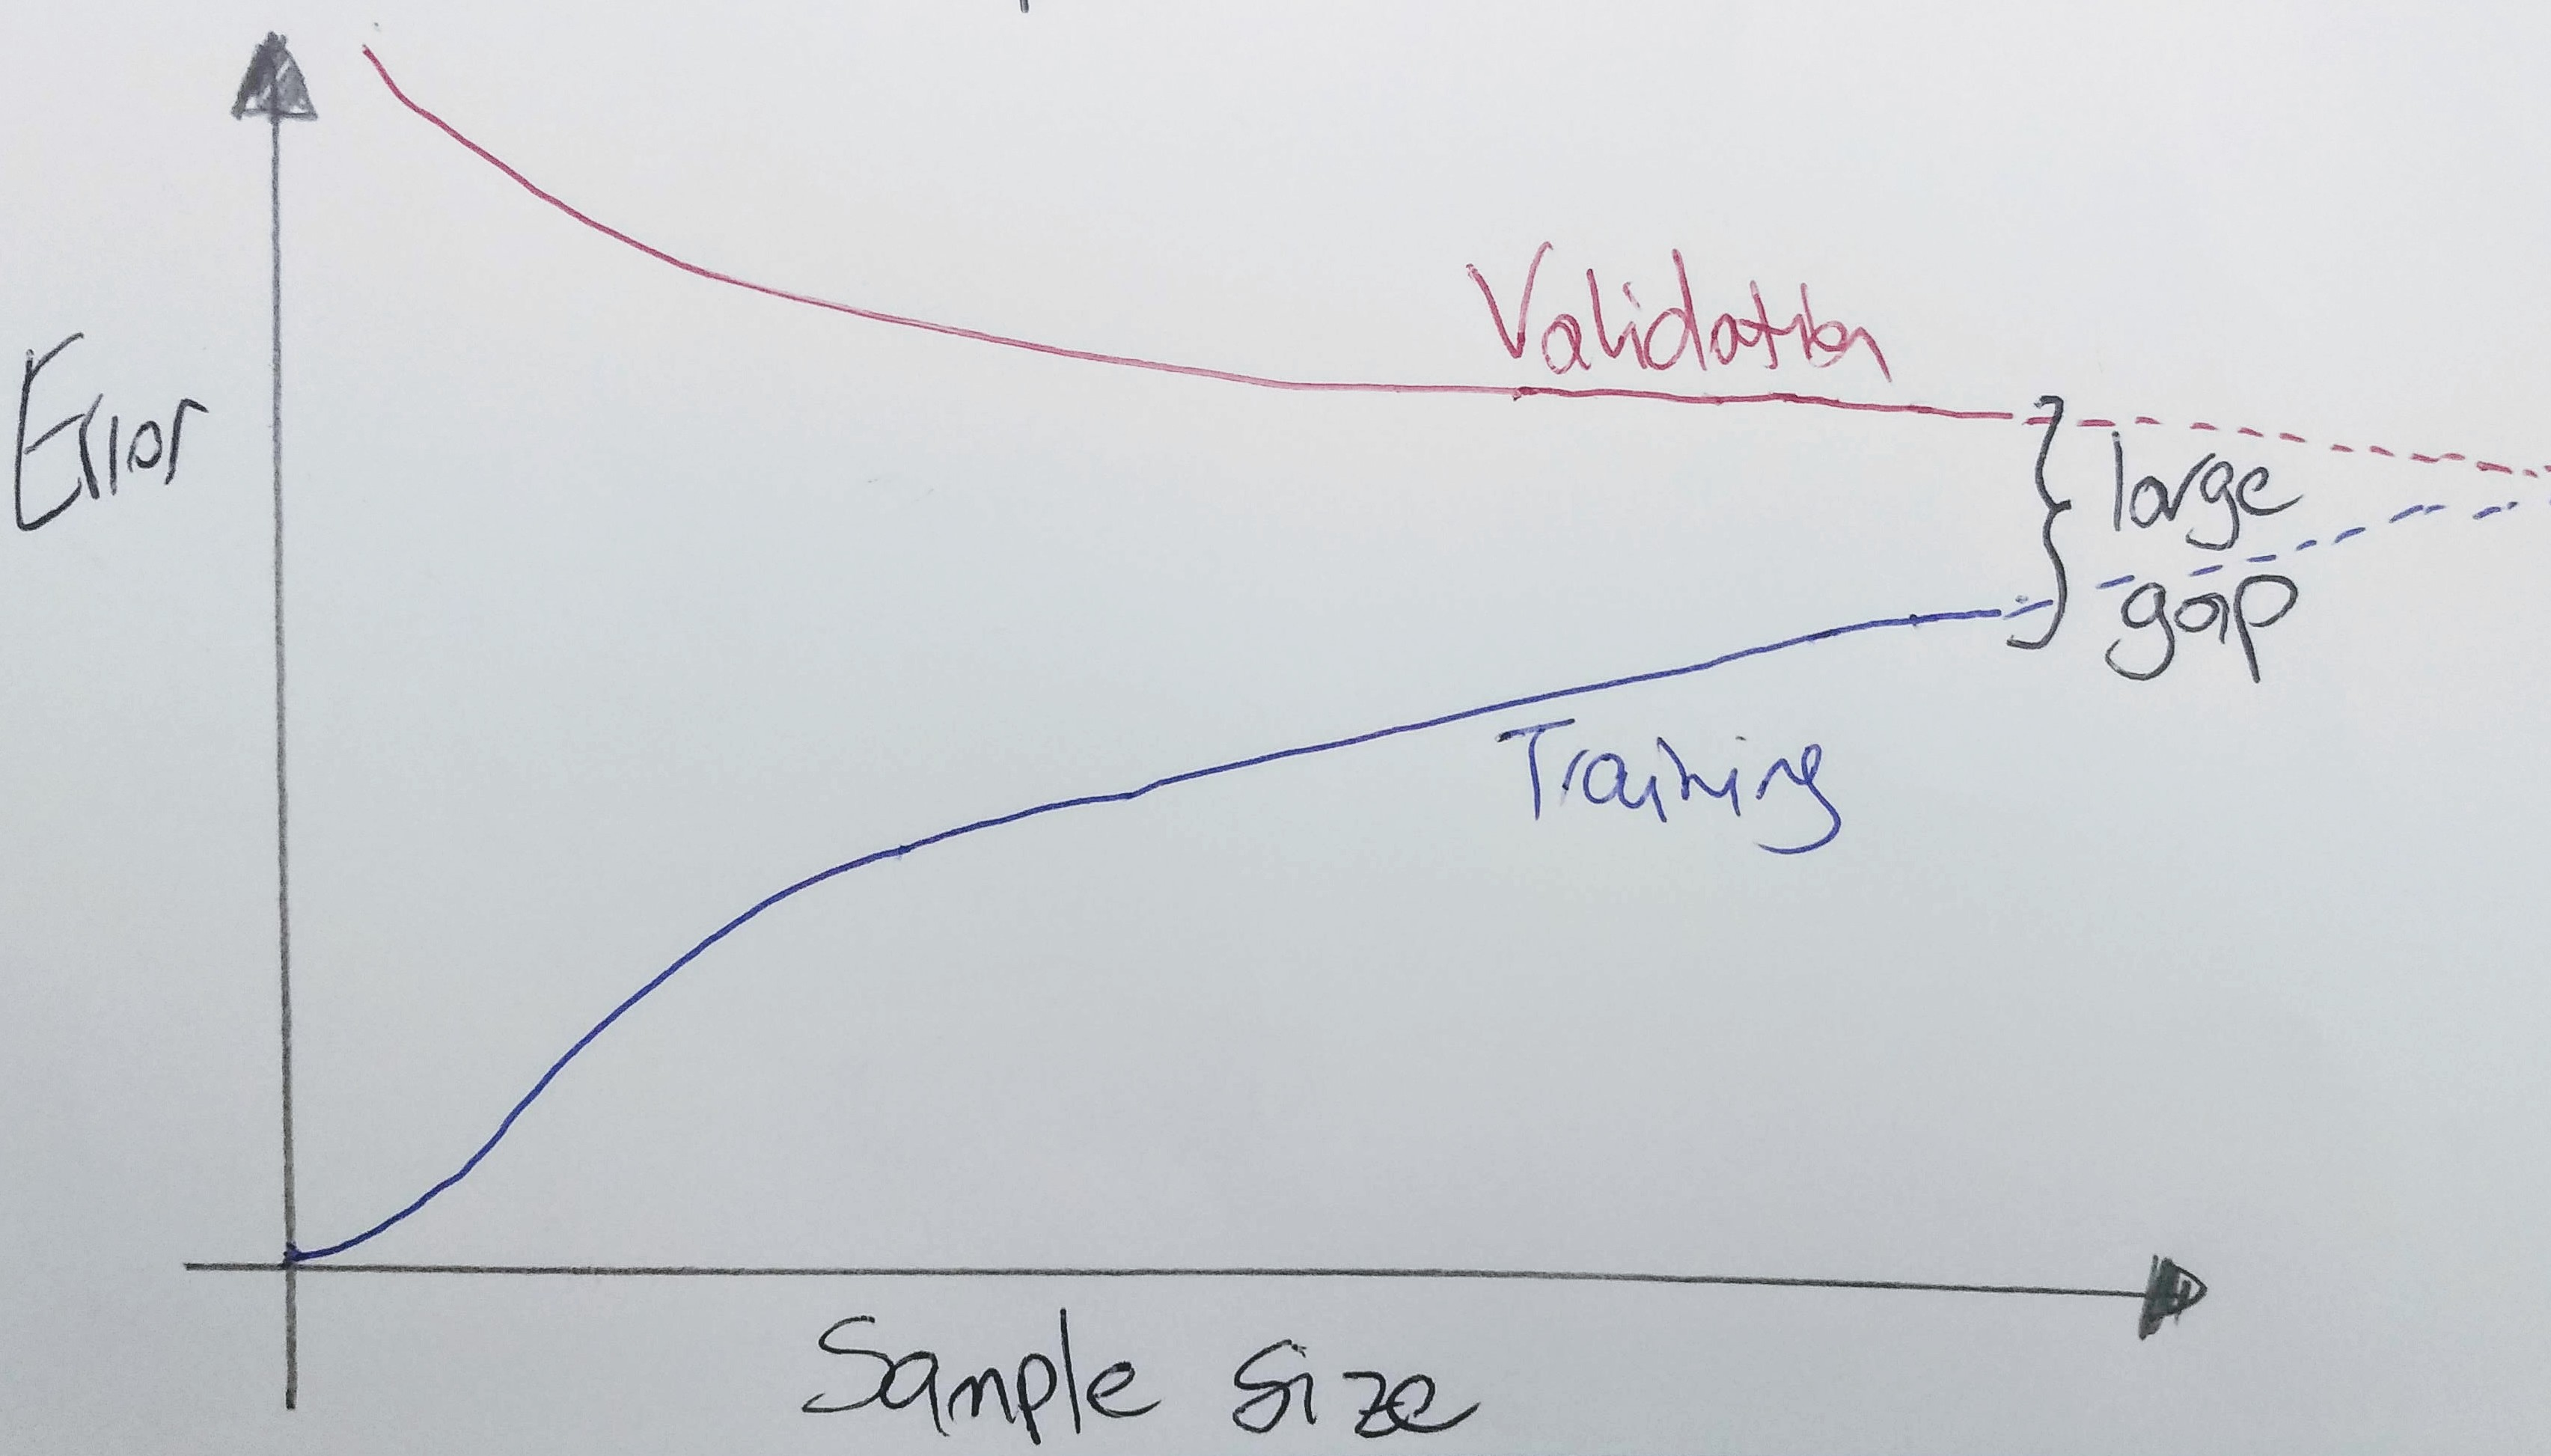
\includegraphics[width=.75\textwidth]{learningcurvevariance.jpg}
\end{center}
\begin{itemize}\addtolength{\itemsep}{0.5\baselineskip}
	\item<2-> Collect more data
	\item<3-> Try a smaller set of ``hand-crafted'' features
\end{itemize} 
\end{frame}

%=============================================================================%
%=============================================================================%
\begin{frame}{High bias}

\begin{center}
		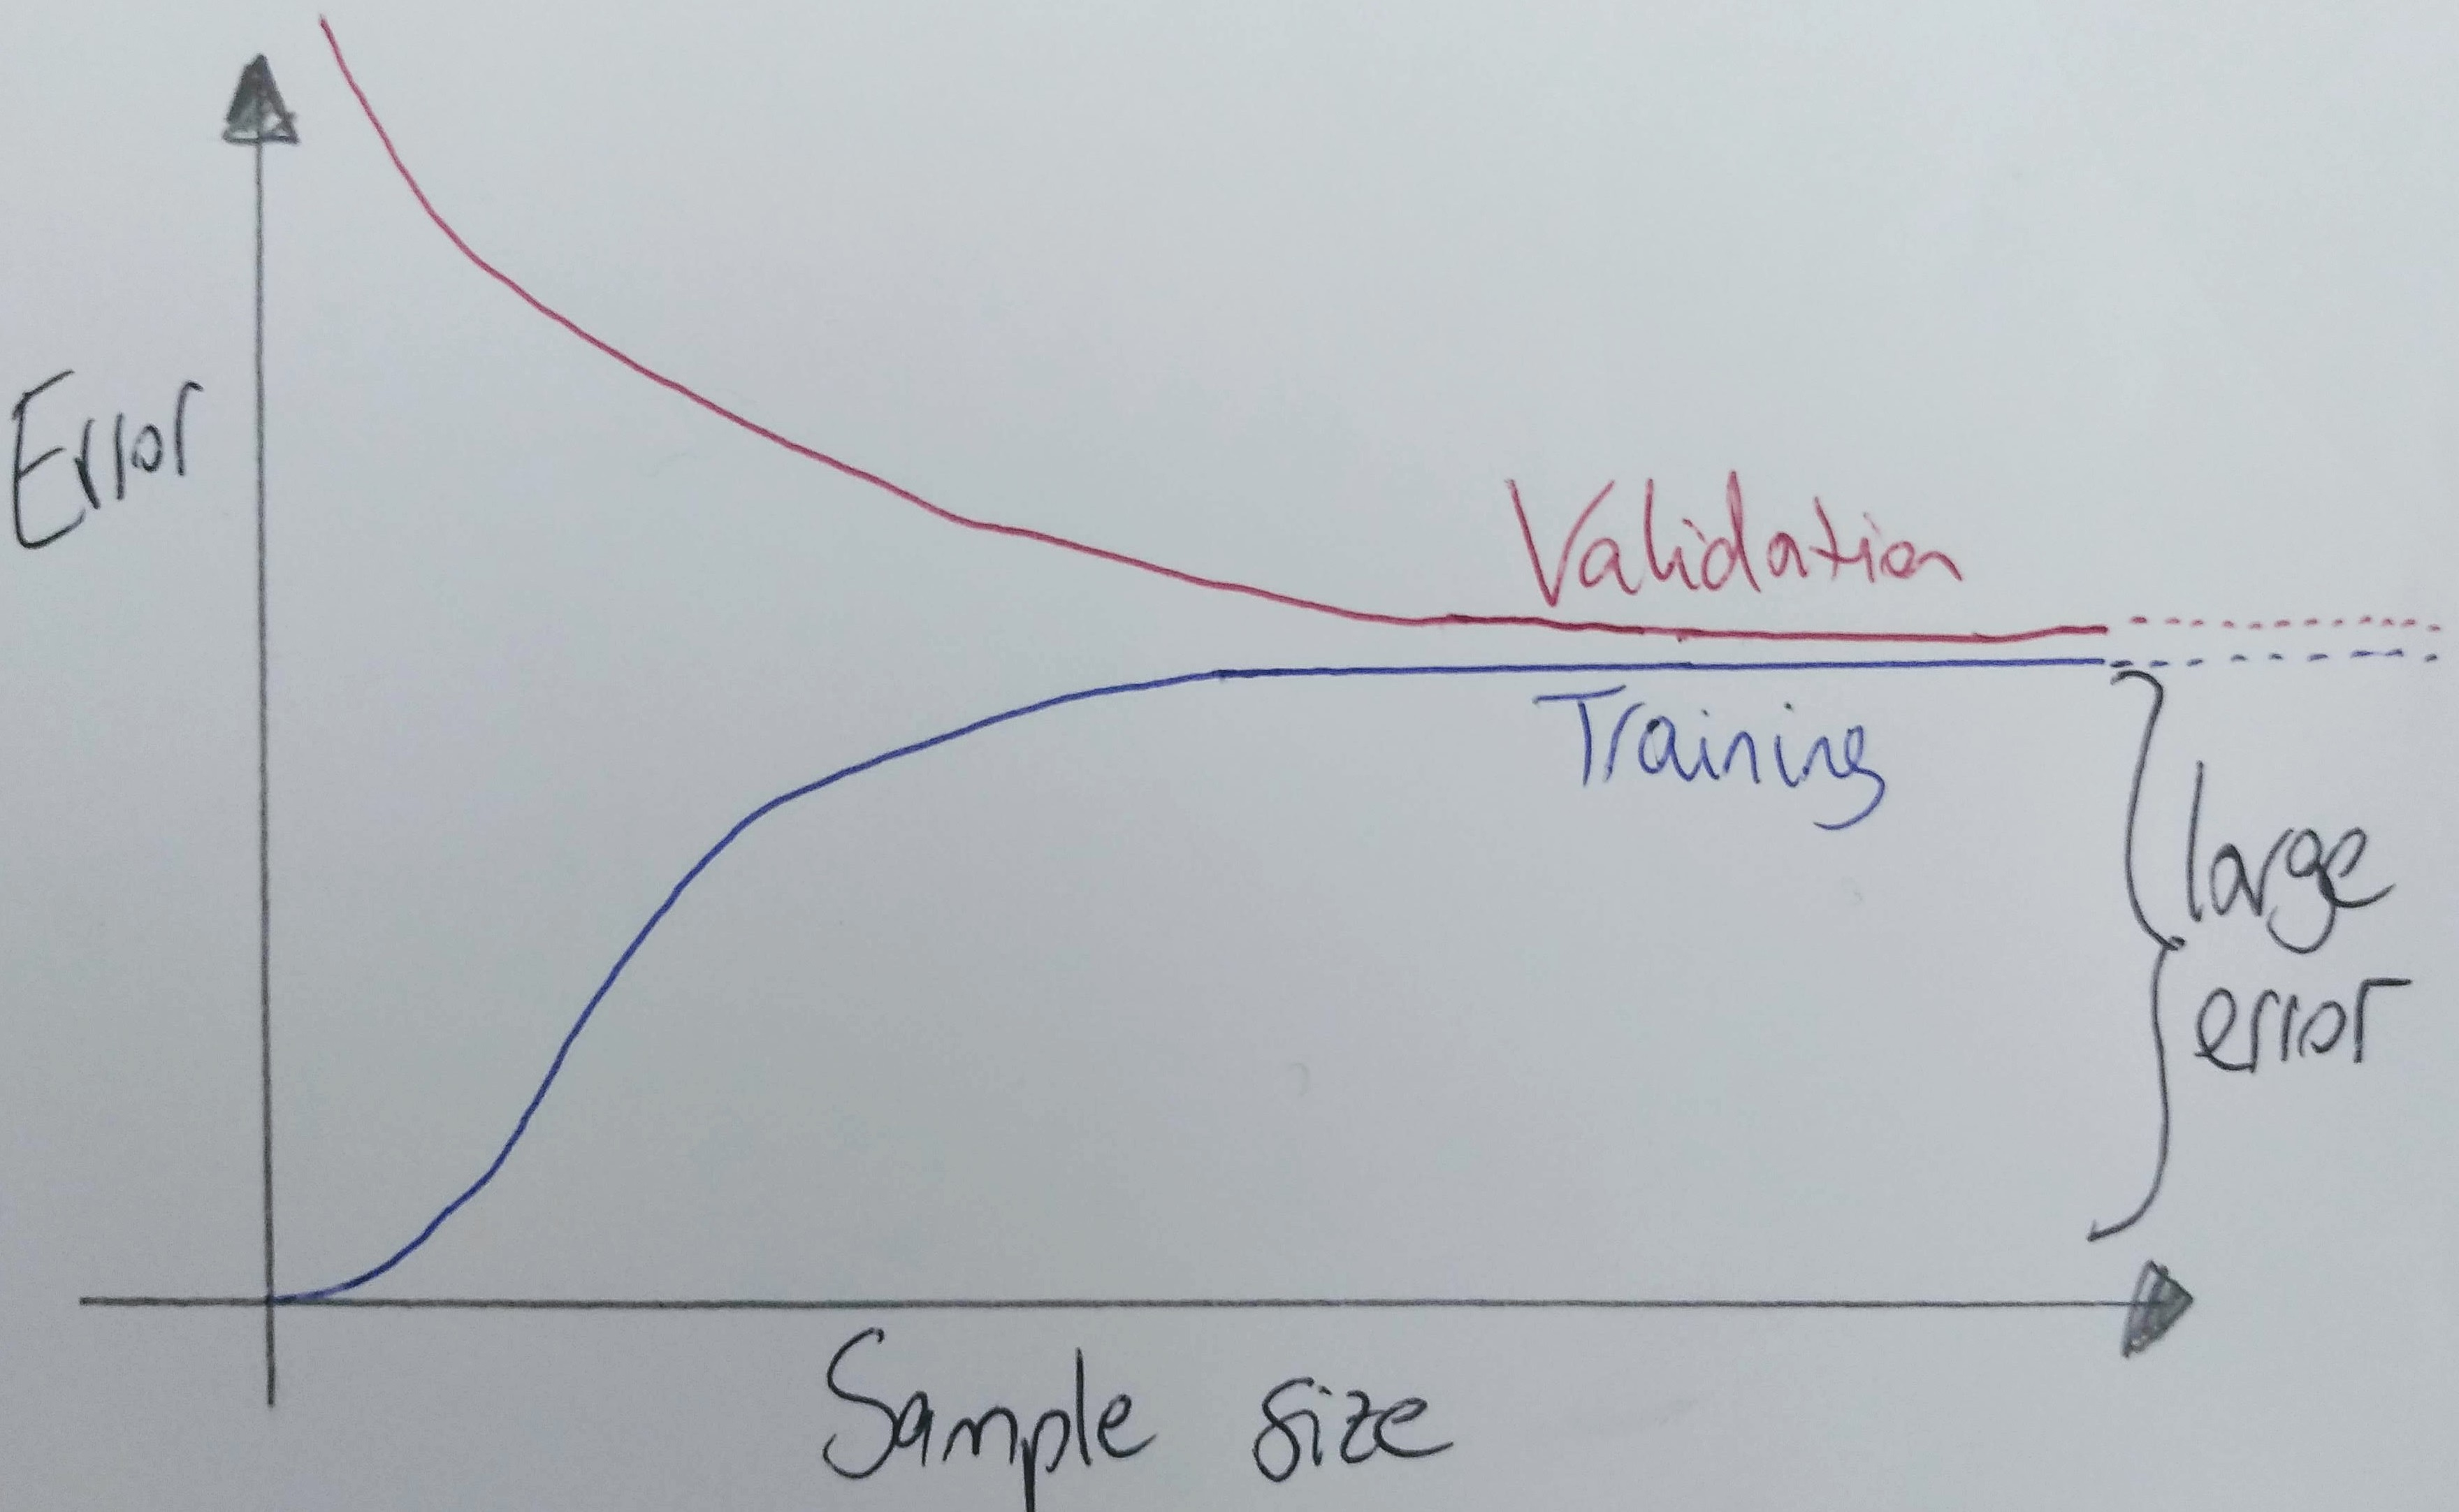
\includegraphics[width=.75\textwidth]{learningcurvebias.jpg}
\end{center}
\begin{itemize}\addtolength{\itemsep}{0.5\baselineskip}
	\item<2-> Try increasing model complexity
	\item<3-> Try additional features
	\item<4-> Add polynomial/splines of features
\end{itemize} 
\end{frame}

%=============================================================================%
%=============================================================================%
\begin{frame}{Which machine learning algorithm should I use?}
 \begin{itemize}\addtolength{\itemsep}{0.8\baselineskip}
	\item A personal choice/what you're comfortable using rather than some rules set in stone
	\item Always start with simple models before using more complex ones
	\item Some methods are more appropriate than others in certain domains:
\end{itemize}
\vfill
\normalsize
\begin{description}\addtolength{\itemsep}{0.4\baselineskip}
		\item [Interpretability:] Decision trees or association rule learning
		\item [Lots of independent features and data:] Na\"{i}ve bayes
		\item [Knowledge of dependencies between features:] Bayesian network
		\item [Thousands of mixed categorical and continuous variables:] Random forests
\end{description}
\normalsize
\end{frame}

%=============================================================================%
%=============================================================================%
\begin{frame}{Which machine learning algorithm should I use?}
\begin{figure}	
	\begin{center}
		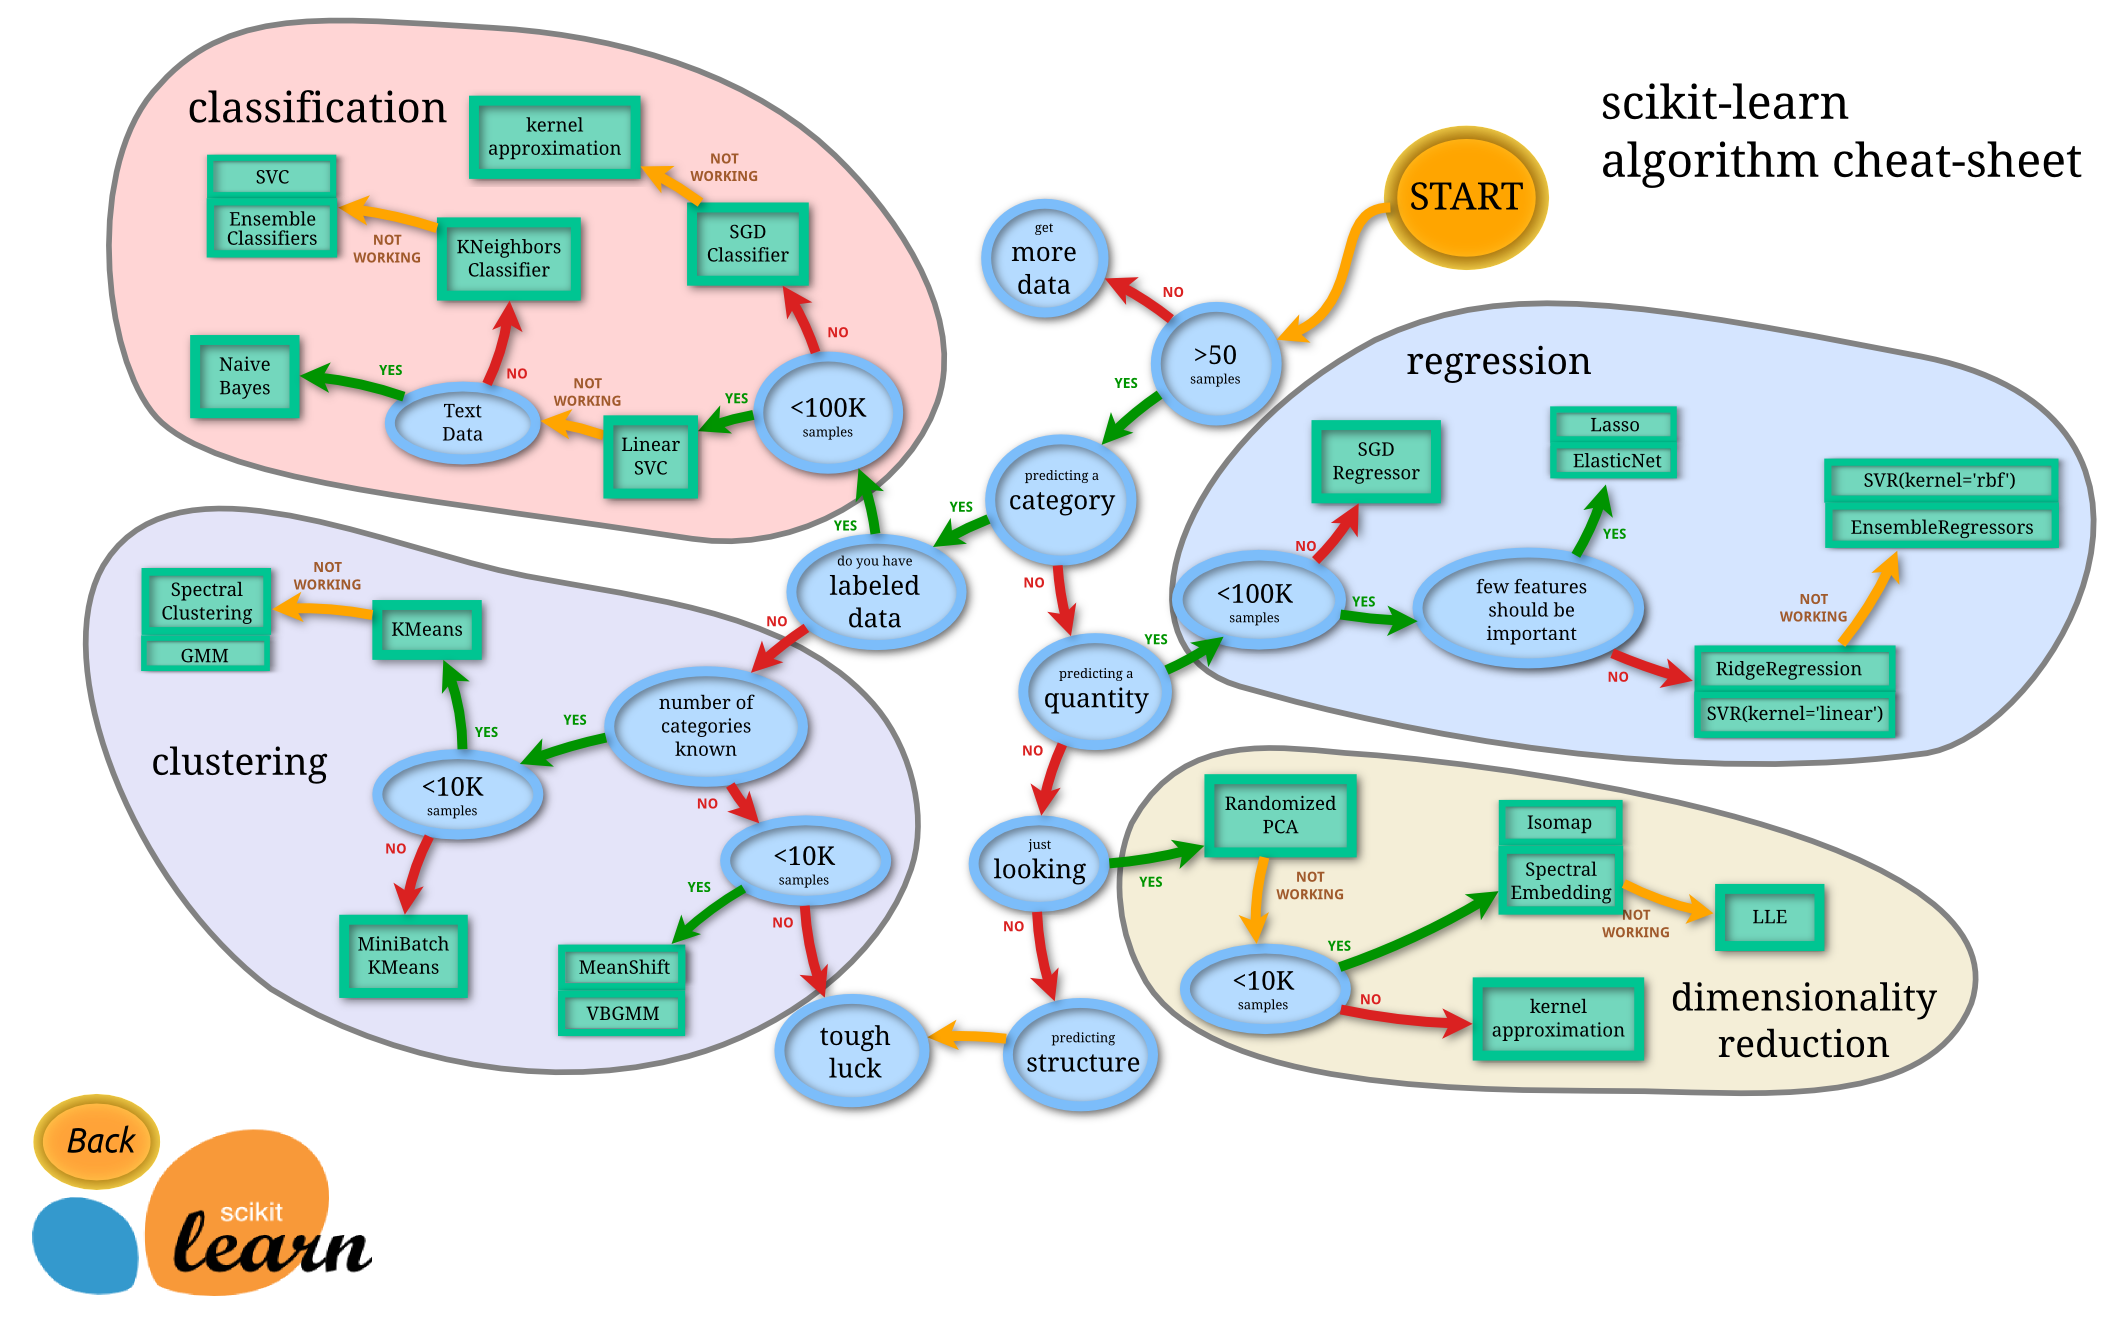
\includegraphics[width=0.9\textwidth]{scikitFlowChart.png}
		\caption{Source: \href{http://scikit-learn.org/stable/tutorial/machine_learning_map/index.html}{scikit-learn.org}}
	\end{center}
\end{figure}
\end{frame}

%=============================================================================%
%=============================================================================%

%=============================================================================%
%=============================================================================%
\end{document}
%=============================================================================%
%=============================================================================%
% End of Document
%=============================================================================%
%=============================================================================%